%----------------------------------------------------------------------------------------
%	Typesetting papers and documents in LaTeX
%----------------------------------------------------------------------------------------

\chapterimage{chapter_head_1.pdf} % Chapter heading image

\chapter{Typesetting documents in \LaTeX}


\LaTeX (pronounced ``lah-tech'' or `` lay-tech'') is a mark-up language that allows an author to specifically, precisely and easily specify how layout and content are combined. It is based on Dr. Donald Knuth's \TeX typesetting system with two goals in mind:\\


\begin{enumerate}
\item It should  be easy a require only a ``minimal amount of effort'' for the author to produce high-quality documents, and
\item It should run on every operating system.\\
\end{enumerate}

Both these goals have been essentially accomplished, resulting in wide-spread use among the scientific community. At this point -- while there are alternatives for typesetting scientific documents  --  \LaTeX\ can easily be considered a basic tool that every physicist should get to know well. Besides making equations look good, the mark-up language is commonly used for:\\


\begin{enumerate}
\item {\bf Making digital and hard-copy media}. This book itself was typeset in \LaTeX.
\item {\bf Making navigable documents by using hyperlinks in a pdf}. This means that you can click on certain words in the document and it will take you to another place in the document, another document, or even a website.
\item {\bf Making high quality documents whose fonts and images can be scaled to be printed on many different kinds of printers}.\\
\end{enumerate}
These features, combined with the fact that the language is open-source and free to use, have made \LaTeX\ a staple in the world of publishing and scientific journals. For instance, many scientific journals prefer or exclusively accept documents in \LaTeX\ code because it is so easy to get to a finished product, and \LaTeX\ documents contain all the information necessary to render the product regardless of platform. If you are considering submitting something to the ArXiv (a well known open-access database for preprints) at some point, you \emph{should} know \LaTeX\ . While you \emph{could} get by without it, very few people do.

%\begin{framed}
{\bf To help you get to know \LaTeX , this book will focus on three things: (1) explaining the basics in what is hoped is a concise way, (2) pointing you towards good online resources on the subject if you're confused and (3) (if you're up to it) helping you to get started with REV\TeX , a package tailored specifically to the needs of physicists.}
%\end{framed}

\section{Getting \LaTeX\ -- compilers and editors}

To use \LaTeX, you need to (1) download the compiler for your operating system, then (2) download a \LaTeX\ editor that you like. The compiler is the program which does the actual typesetting by creating a \texttt{.pdf} file, and it is different for every operating system:\\
\begin{enumerate}
\item Microsoft Windows $\implies$ MikTeX: \url{http://miktex.org/}
\item Mac OS $\implies$ MacTeX: \url{http://tug.org/mactex/}
\item Linux $\implies$ look for the \texttt{texlive} package in your package manager.\\
\end{enumerate}
There are \emph{many} \LaTeX\ editors, each of them has its own advantages and disadvantages. Some of the favorites at UT are \footnote{This book was typeset using Texmaker. The hotkeys and structure manager came in very handy when working through a lot of code and trying to manage multiple chapters.}:
\begin{figure}[h]
\centering
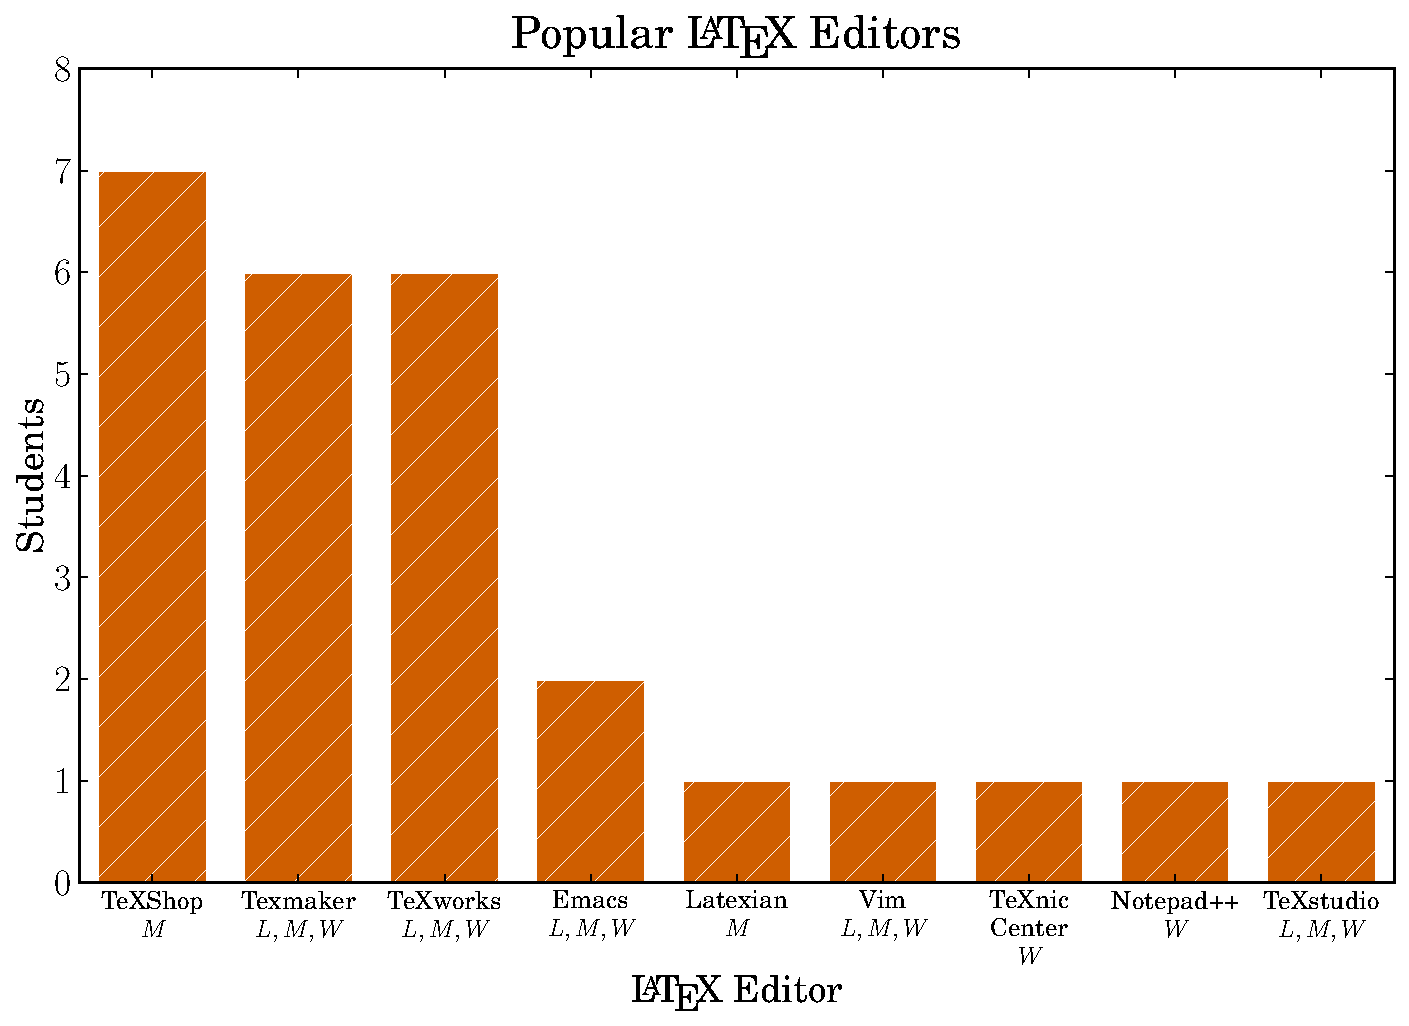
\includegraphics[scale=.675]{editorprefs.pdf}
\caption{A Facebook survey was taken of other UT SPS students' \LaTeX\ editor preferences. The plot above documents the results. Under each editor name, the italicized capital letters show which operating systems the programs are compatible with:  $L$ for Linux, $M$ for Mac OS X, and $W$ for Windows. If you choose one of these, you are most likely to find someone else who knows about the editor you're using (in case you get lost). \emph{Note:} Emacs, Vim, and Notepad++ are text editors that can be modified to run \LaTeX\ code. If you're a serious programmer you may already know what these are. If you're new to \LaTeX\ , it might be best to try something else first.}
\end{figure}

A good compare and contrast of some of the different \LaTeX\ editors out there can be found at \url{http://en.wikipedia.org/wiki/Comparison_of_TeX_editors}

\section{Getting started immediately }
This section is intended to be short and the absolute minimum to get you started with writing a paper in \LaTeX . If you are more interested in a comprehensive introduction you should \emph{certainly} check out these two much more complete guides:

\begin{description}
\item[The \LaTeX\ Wikibook] Found at \url{http://en.wikibooks.org/wiki/LaTeX}, this is probably the best organized and easiest to navigate website. It is slightly more encyclopedic and useful for troubleshooting.
\item[The Not So Short Introduction to \LaTeX 2e] If you're interested in having a \texttt{.pdf} or book reference, \url{http://tobi.oetiker.ch/lshort/lshort.pdf} is a great document that has a lot in common with The \LaTeX\ Wikibook, but is typeset entirely in \LaTeX\ and has a bit more of an attitude.
\end{description}

Both of these references are very similar, and are very enlightening. For a more full understanding of \LaTeX\ (it would be senseless to try to compete with them) you should definitely spend a few hours reading through them. To get writing immediately refer to the document and explanation below.

\subsection{A basic document}
An example of a simple yet functional basic document that has title, abstract, some organization and an equation:


\begin{framed}
\begin{verbatim}
% This is a comment because nothing after a % sign can be displayed. 
\documentclass{article}
\title{This is a title}
\author{Name}
\date{\today}

\begin{document}
\maketitle
\begin{abstract}
This is my abstract
\end{abstract} 
\begin{section}{This is a section}
\begin{subsection}{This is a subsection}
Here is text and below is an equation:
\begin{equation}
\hat H = - \frac{\nabla^2}{2} - \frac{1}{x}
\end{equation}
\end{subsection}
\end{section}
\end{document}
\end{verbatim}
\end{framed}

This code needs to be run for the compiler to yield a document. When run in a \LaTeX\ editor the code produces output that looks like this:

\begin{figure}[H]
\centering
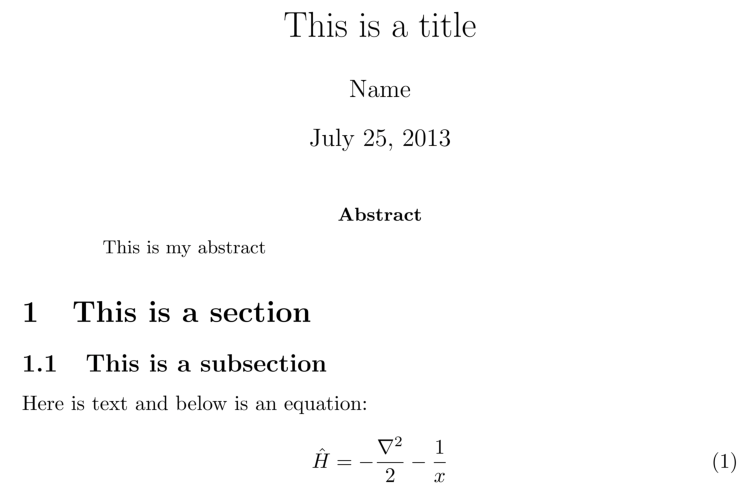
\includegraphics[scale=1]{ex1_crop2.pdf}
\end{figure}
\subsection{Commands and environments}
To understand how this file made it to output, let's look at the general features of the file. First of all, notice that  every word that has a \textbackslash\ in front of it is not displayed. This is because commands in \LaTeX\ start with a backslash. Commands represent blocks of code in \TeX\ , the underlying language that is run to create and render all of the typeset objects that you see in the output document.
Second, notice that every time there is a command of the form \verb|\begin{|  {\it environment} \verb|}|, there is another of the form \verb|\end{| {\it environment} \verb|}| some time later. This is because these commands delimit ( set the bounds of ) blocks of code called ``environments". Environments are spaces in which all code is interpreted in a specific way. Some commands and environments therefore only make sense or can be used within certain kinds of environments. By thinking in terms of {\it commands} and {\it environments}, \LaTeX\ translates a few words into a lot of specific \TeX\ commands that we would really rather not see (because they are incredibly tedious). This is why the system is so powerful: you only need to give \LaTeX\ your content, and it does all the formatting according to rules you can understand and tinker with. {\bf Learning how to use the system well is therefore really just a matter of understanding how the existing rules work and how new rules are made.}



\section{How the existing rules work}

The undisputed best way to understand how the rules of \LaTeX\ work is to actually try to write some files. While this is true, it is handy to know about the basic structure and conventions of a \texttt{.tex} document when searching for documentation and for imitating examples found online. This section will therefore cover the structure of \LaTeX\ through the lens of the basic document above.

\subsection{The structure of a \LaTeX\ document}\label{structureoflatex}
Every document starts by choosing what class of document it is (is it an article? a letter? a book?) . This is done in the example with the \verb|\documentclass{article}| command. When \LaTeX\ sees this command it looks for a specific \texttt{.cls} file that has all of the basic formatting information. In the example, it looked for \texttt{article.cls} and obtained valuable information like the paper size, font sizes, and other environments and commands used in the document. This roughly constitutes the `lowest-level' of code, and contains a lot of \TeX\ code. You {\it do not} want to mess with these class files unless you have a lot of practice and no existing project can be modified to suit your needs (very rare).

In general, the class file will also load packages in the \texttt{.sty} file format. These are higher level files that are usually task-specific and contain even more commands and environments. For instance, \texttt{hyperref} is a package which allows for hyperlinks to websites, files, or other parts of the document. Packages are loaded using the \verb|\usepackage{}| command (e.g. \verb|\usepackage{hyperref}|) between the \verb|\documentclass{}| command and \verb|\begin{document}| in what is referred to as the \emph{top matter} or \emph{preamble}. The preamble is very important because it is where all of the extra functions you might want to use are added. For instance, if you want to change the way the title formatting looks or want to define a function to get rid of the tedium or repeating code, the preamble is the place to put this code. 

% PUT A LINK HERE TO THE CODING NEW FUNCTIONS SECTION
 Once the compiler sees \verb|\begin{document}| the preamble is over and everything it reads is document content -- no more commands and environments may be added or defined. When it gets to \verb|\end{document}|, that's the end of the file and the \LaTeX\ compiler will not evaluate anything past it.
\subsection{Anatomy of our basic example}
\hfill \\
\begin{center}
\begin{flushright}
{\large  \avantfont Commands used in the example}
\end{flushright}
{\renewcommand{\arraystretch}{1.2}
    \begin{tabular}{  | p{3.5cm } | p{11.5cm}|}
   \hline \hline
	\verb|\documentclass[]{}|		&    {\bf loads the class file for the document which contains the basic information (commands and environments) the program needs to start typesetting your code} and is at the start of every \LaTeX\ document. This basic information is information like what size paper you're using, whether you're writing something long like a book or short like a letter, and whether you'll be using a lot of complicated symbols. All these things have an impact on what kinds of tools the program will need to do the job correctly.  In general, the class file will therefore have options that you put in the \texttt{[]} for these kinds of things and so it will look more like \verb|\documentclass[11pt, letterpaper]{article}|.\\ \hline
	\verb|\title{}|						&  stores the title information so that the \verb|\maketitle| command can use it later.\\ \hline
	\verb|\author{}|					&  stores the author information so that the \verb|\maketitle| command can use it later.\\ \hline
	\verb|\date{}|						&  stores the date information so that the \verb|\maketitle| command can use it later.\\ \hline
	\verb|\today|							&  retrieves the current date and outputs according to a certain format. This command can be put anywhere that text can be placed. \\ \hline
	\verb|\maketitle|					&  renders a title using information from \verb|\title{}|, \verb|\author{}|, \verb|\date{}|\\ \hline
	\verb|\hat|								&  puts a hat symbol over the next symbol in the equation : e.g. $\hat \alpha$ , $\hat 3$, $\hat r$\\ \hline
	\verb|\frac|							&  makes a fraction with the first \texttt{\{\}} defining the numerator, and the second \texttt{\{\}} defining the denominator \\  \hline
	\verb|\nabla|							&  makes a del (nabla) symbol that looks like $\nabla$ \\ \hline
    \end{tabular}	}	
\end{center} 
\hfill \\ 

\newpage
\begin{center}
\begin{flushright}
{\large  \avantfont	 Environments used in the example}
\end{flushright}
    \begin{tabular}{  | p{2cm } | p{13cm}|}
     \hline \hline
\texttt{document} & contains the contents of the document. This means it contains the other environments. It also means that anything after \verb|\end{document}| will not be typeset.\\ \hline
\texttt{abstract} & interprets its contents as text that contains the abstract of an article. As an environment it formats the contents to look a certain way: changes the margins and font to look like an abstract.\\ \hline
\texttt{section} & interprets its contents as body material and makes a title for the section based on the number of sections before it. The environment assumes that the first \texttt{\{\}} it sees contains the title for the section. Therefore, since no section preceded the one in the example, the section was formatted as `1 This is a section'.\\ \hline
\texttt{subsection}& interprets its contents as body material and makes a title for the subsection based on the number of subsections before it and the section it's in. \\ \hline
\texttt{equation} & interprets its contents in math mode. This means that it interprets text as a string of a variables unless it is a command like \verb|\hat| or \verb|\frac{}{}|.\\ \hline  
    \end{tabular}		
\end{center}

\subsection{Basics continued: text \& math modes}
In text mode, you delimit the math environment by using \$ signs. This means that whenever you want to put in a symbol, subscript, or equation into a sentence you can easily do that by wrapping the content in dollar signs.
\begin{corollary}[Math in text mode]
\hfill
\begin{framed}
\texttt{Einstein's famous equation} \verb|$ E = mc^2$| \texttt{was not rigorously proven by Einstein, but rather by the mathematician Felix Klein.} 
\end{framed}
produces
\begin{framed}
Einstein's famous equation $ E = mc^2$ was not rigorously proven by Einstein, but rather by the mathematician Felix Klein. 
\end{framed}

\end{corollary}
Some environments, like the \texttt{equation} environment we saw before, will be in math mode automatically. If you want to put text inside an equation, use the \verb|\text{}| or \verb|\mbox{}| commands to get into text mode.

\begin{corollary}[Text in math mode]
\hfill
\begin{framed}
\begin{verbatim}
\begin{equation}
\Delta E = E_{\text{Final}} - E_{\mbox{Initial}}
\end{equation}
\end{verbatim}
\end{framed}
produces
\begin{framed}
\begin{equation}
\Delta E = E_{\text{Final}} - E_{\mbox{Initial}}
\end{equation}
\end{framed}
As you can see, both \verb|\text{}| or \verb|\mbox{}| are effective in putting text into the equation, { \bf but only  \verb|\text{}| properly does subscripts and superscripts.}
\end{corollary}

Whichever mode you're in, extra spaces and extra line breaks are ignored. This helps reduce syntax ambiguity and helps writers visually organize separate content in the \texttt{.tex} without impacting how the file output looks when file is run.



\section{Getting more packages}\label{packagemanagers}

As we've seen so far, \LaTeX\ is just a way of automating the underlying \TeX\ language by use of commands and environments that summarize a lot of dirty work we don't want to do. There are a lot of writers over the years who have decided do more work to create and increasing number of packages full of more commands and environments to make their lives easier. The good news is that since \LaTeX\ is open source, everyone can use and has access to those packages. These packages are used for inserting pictures, doing complicated referencing, and even making animations. This is partially why \LaTeX\ is so great for scientists -- it's open, automates repetitive tasks, and continuously improves.

Since you probably have to make use of these packages, you will have to use the \verb|\usepackage| command mentioned briefly in section \ref{structureoflatex}. When you installed \LaTeX\ however, you might not have installed all the packages you need. This is natural and unavoidable since new packages are written every day. To get at these packages though, the easiest thing to try first is just to use the by far is to use  \verb|\usepackage| command. If you have a good \emph{package manager}, it will go find the package for you and install it. If you do not have such luck, you can access the package managers directly: 
\begin{enumerate}
\item MiK\TeX 's package manager is called MiK\TeX\ Package Manager (MPM) appropriately enough. You can get to it through the start menu (it'll say ``Browse Packages'') on PC.
\item Mac\TeX 's package manager is called \TeX\ Live Utility, and can be accessed through the Applications folder on a mac.
\end{enumerate} 


\section{More basics: Tables, Figures and References}
Now that you know how to write math in text mode and text in math mode, you are essentially ready to write papers. The three most common things you'll probably want to know about after that are (1) how to make tables, (2) how to put figures in a document and (3) how to reference things (other papers, figures, equations, etc.).  For this you may need to use some new packages as explained in 

\subsection{To make a table} Look at the code examples at \url{http://en.wikibooks.org/wiki/LaTeX/Tables#Basic_examples}. The gist of it is that you have to give \LaTeX\ some instructions about how to align and seperate the columns, and tell it where each cell is (using the \verb|&| alignment character) and where each line ends (using \verb|\\| ). You can divide up rows using the \verb|\hline| command.
\subsection{To add figures}

In \LaTeX , you either import some picture file by grabbing it with some code, or you create a picture with some code. The most common thing physicists do is import picture files, since making pictures is very complicated. The easiest thing to do to import pictures is to make a folder with the picture files in it, and then put it in the same folder as your \texttt{.tex} file. That way, wherever the folder containing your document goes, your pictures will follow. 

There are a few picture formats you can use, but you want to use \texttt{.pdf} or \texttt{.eps} since they are vector graphics and don't look cruddy when you change their scale factor.{\bf To learn how to use figures, read \url{http://en.wikibooks.org/wiki/LaTeX/Floats,_Figures_and_Captions} and use one of their examples}.

\begin{remark}
One of the most common problems people have with figures is getting them to go in the right place. \LaTeX\ by default searches for a good place to put it based on the density of text you have, but you can make it bend to your will by using placement specifiers:

\url{http://en.wikibooks.org/wiki/LaTeX/Floats,_Figures_and_Captions#placement}

Basically, with the \texttt{float} package you can tell \LaTeX\ to put the figure exactly where you say. Sometimes this doesn't look so great, since the spacing isn't optimized for word density, but sometimes it's necessary. 
\end{remark}

\subsection{References}

One thing \LaTeX\ makes easy for scientists is citing references, making footnotes\footnote {Making footnotes is as easy as putting \texttt{\textbackslash footnote \{some text\}} exactly where you want the footnote to show up on the page.}, referring to equations and figures in their documents, and referring to websites. 

\subsubsection{Referencing other parts of your document}
The most general and versatile command for labelling things for referencing is \verb|\label{marker}|:\\ \url{http://en.wikibooks.org/wiki/LaTeX/Labels_and_Cross-referencing}
With this labelling command you can label just about anything. To use it all you have to do is give whatever you're labelling a name (a marker) and then use the \verb|\ref{marker}| to reference it later. For instance if you have an equation below:
\begin{equation}\label{1ecorehamiltonian}
\hat H^{\text{core}}(1) = -\frac{1}{2}\nabla^2_1 - \sum_\alpha \frac{Z_\alpha}{r_{1\alpha}} 
\end{equation}
You can label it like so:
\begin{framed}
\begin{verbatim}
\begin{equation}\label{1ecorehamiltonian}
\hat H^{\text{core}}(1) = -\frac{1}{2}\nabla^2_1 - \sum_\alpha \frac{Z_\alpha}
{r_{1\alpha}} 
\end{equation}
\end{verbatim}
\end{framed}
Now whenever you say \verb|\ref{1ecorehamiltonian}| anywhere in text mode, ``\ref{1ecorehamiltonian}'' shows up. With this method, no matter how many equations you have, the equation number will be matched to the reference and you won't have to go through and tweak the numbers.

\begin{remark}
When you label a figure, be sure to put the label command \emph{after} the \verb|\includegraphics{}| command, or else the numbers will be screwed up!
\end{remark}
\subsubsection{Citing other authors}
Citing authors can be complicated, but the \LaTeX\ wikibook online has very good coverage of this topic:

\begin{enumerate}
\item If you're looking for something easy, use the \texttt{thebibliography} environment found at

 \url{http://en.wikibooks.org/wiki/LaTeX/Bibliography_Management#Embedded_system} 
\item If you're looking for a professional solution, use Bib\TeX\:

\url{http://en.wikipedia.org/wiki/BibTeX}.
\end{enumerate}

\section{Templates in \LaTeX\ }

The easiest way to get started with a new proiect is to download an appropriate template and to experiment with it. A very basic template for writing papers was written by Jonathan Blair and can be found at the SPS website -- \url{http://www.ph.utexas.edu/~sps/}. More complicated templates can be found all over the internet. 
\hfill \\
\begin{center}
\begin{flushright}
{\large \avantfont Template websites}\\
\end{flushright}

\begin{tabular}{|p{7cm} | p{8.5cm}| }
\hline
\hline
\url{http://publish.aps.org/revtex} & The standard class file for in publishing \\ \hline
\url{http://www.latextemplates.com/} & Best for books and modern styling. \\ \hline
\url{http://www.howtotex.com/templates/} & More templates -- more of the same \\ \hline
\url{https://www.sharelatex.com/templates/} & Great assortment of article styles\\ \hline

\end{tabular}
\end{center}

\chapterimage{chapter_head_1.pdf} % Chapter heading image

\chapter{ More advanced features of \LaTeX}
\section{Creating new commands and environments}
Since \LaTeX\ is a programming language, you can make new commands.

\subsection{Simple Substitutions}
Use the
\begin{verbatim}
\def\function_name{value}
\end{verbatim} command in the preamble to define a simple substitution. Anywhere \LaTeX\ sees 
\begin{verbatim}
\function_name
\end{verbatim}, \texttt{value} will appear.

\subsection{Functions with Parameters} Use the 
\begin{verbatim}
\newcommand{\cmnd_name}[num_vars]{...#n...}
\end{verbatim}  in the preamble. Again, \texttt{\textbackslash cmnd\_ name} is the new function name, but you can tell \LaTeX\ how many variables  you want, then use them to create 
a full``macro" to substitute, using \# n to get the value of the n-th variable.

\begin{example}[Dirac Notation] \hfill \\ Say for instance you were doing a lot of quantum mechanics and you wanted to be able to write bras, kets, and brakets very simply. You might want to do this since you might like your equations to be easy to read when you write them and writing it out is somewhat verbose. To make a braket command, you could type.
\end{example}




%\subsection{Class files}
% This command is at the start of every \LaTeX\ document. {\bf It loads the class file for the document which contains the basic information the program needs to start interpreting your code}. This basic information is information like what size paper you're using, whether you're writing something long like a book or short like a letter, and whether you'll be using a lot of complicated symbols. All these things have an impact on what kinds of tools the program will need to do the job correctly.  In general, the class file will therefore have options for these kinds of things and will look more like \verb|\documentclass[11pt, letterpaper]{article}|.
% 
% \begin{remark}
% Because class files can be tailored to specific applications, some scientific publishers have their own class files that anyone can download. The American Physical Society has a class file called \texttt{revtex4-1} which contains all the formatting information they use to make journals like \emph{Physical Review Letters} and \emph{Reviews of Modern Physics}.
% \end{remark}
%\subsection{The preamble}
%The space between the \verb|\documentclass{...}|  and \verb|\begin{document}| is special and called the \emph{preamble}. It's special because this is where all the functionality (commands and environments) not defined by the class file come into play.  \emph{packages} using commands like e.g. \verb|\usepackage[graphicx]|.
%
%\subsection{The document}
%Once inside the \verb|\begin{document}| environment, other commands and environments come into play. In our case, the first thing we see is \verb|\maketitle|, which constructs the title from parameters set in the preamble. Next, we come to our first environment ( \verb|\begin{abstract}| ). This environment looks at the text inside it and typesets it at the top of the page with a particular fontsize and margin size. That's all it does. To prove this to yourself you can copy and paste the whole environment over and over and make 5 abstracts if you want. 

\section{Installing REV\TeX}

By now, if you have written a bit of code and browsed the wikibook, you probably have a pretty basic and functional understanding of \LaTeX\ and can format papers in the \texttt{article} class pretty well. To make it easier for physicists to write papers and to standardize formatting in the APS and AIP journals, APS has released a package they call REV\TeX. The samples in this public package both look great, and have excellent documentation embedded in the documents. To install: \\

\begin{enumerate}
\item Look in your package manager (section \ref{packagemanagers}) and install REV\TeX. It probably shows up in your package manager as \texttt{revtex4-1}. 
\item Go to the SPS webpage and download the UTSPS REV\TeX\ Sample Pack.
\item When you unzip this file, it will contain three folders
\begin{description}
\item{aapm} contains a sample \texttt{aapmsamp.tex} and a template \texttt{aapmtemplate.tex} from the American Association of Physicists in Medicine.
\item{aip} same documents instead from the American Institute of Physics
\item{aps} same documents instead from the American Physical Society.
\end{description}
\end{enumerate}
After you are done unpacking, these files can be excellent references for producting high-quality reports and can be very valuable all-encompassing references if you are just writing a paper. The wikibook is a great way to learn \LaTeX\ in general, but these official APS and AIP documents are excellent templates for PHY 353L or PHY 474.


